\section{Greedy Deployment}
\label{sec:greedy_deployment}

In this scheme, we deploy the largest reactor first until another
deployment of that reactor exceeds the demand---as outlined in
\ref{fig:greedy_diagram}. Then we move to the next largest reactor until the
next deployment of the smallest capacity reactor exceeds the
demand. This scheme is not a proxy for strategic decisions by individual
actors it merely meets the demand in a roughly efficient manner.

Previous work from Bachmann et al. \cite{bachmann_enrichment_2021}
employed a similar scheme to explore the deployment of advanced
reactors in the \gls{usa}. This scheme is computationally efficient and allows
for the exploration of the deployment of advanced reactors in a way that is not
overly complex. This scheme is most useful for scenarios where the user is
interested in comparing metrics relative to the number of specific reactors
deployed outside of the context of the problem.

\begin{figure}[!htbp]
    \centering
    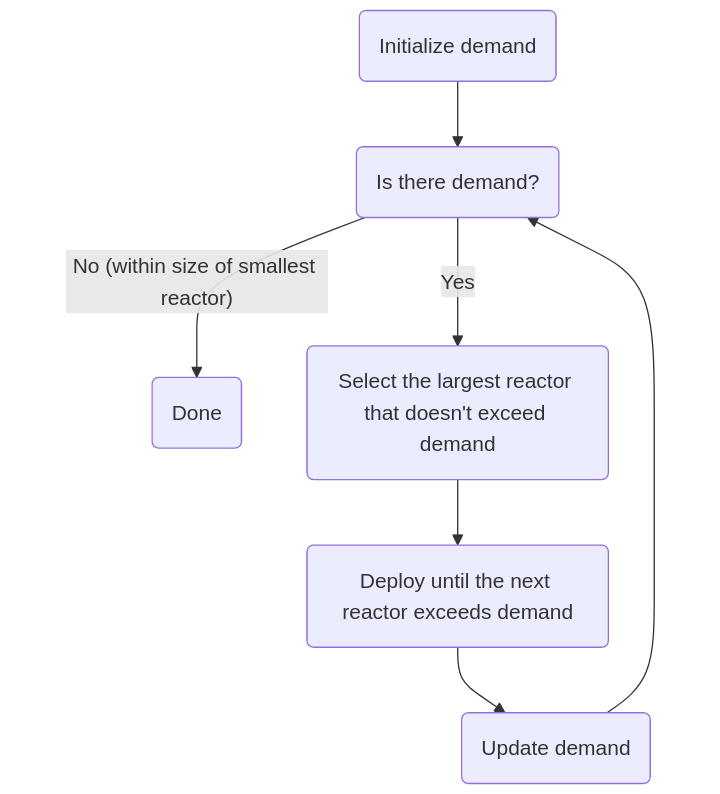
\includegraphics[scale=0.4]{images/schemes/greedy_diagram.png}
    \caption{Greedy Deployment Diagram}
    \label{fig:greedy_diagram}
\end{figure}

Through the greedy deployment, we are not attempting to capture the complexity
of the deployment problem but rather to explore the implications of deploying a
certain number of reactors. As such, we limit the discussion of realism to the
extent that the scheme meets the demand and could mirror large actors in a
market. The scheme will deploy reactors until the demand is met within the
amount of the smallest capacity reactor.

